\documentclass[1p]{elsarticle_modified}
%\bibliographystyle{elsarticle-num}

%\usepackage[colorlinks]{hyperref}
%\usepackage{abbrmath_seonhwa} %\Abb, \Ascr, \Acal ,\Abf, \Afrak
\usepackage{amsfonts}
\usepackage{amssymb}
\usepackage{amsmath}
\usepackage{amsthm}
\usepackage{scalefnt}
\usepackage{amsbsy}
\usepackage{kotex}
\usepackage{caption}
\usepackage{subfig}
\usepackage{color}
\usepackage{graphicx}
\usepackage{xcolor} %% white, black, red, green, blue, cyan, magenta, yellow
\usepackage{float}
\usepackage{setspace}
\usepackage{hyperref}

\usepackage{tikz}
\usetikzlibrary{arrows}

\usepackage{multirow}
\usepackage{array} % fixed length table
\usepackage{hhline}

%%%%%%%%%%%%%%%%%%%%%
\makeatletter
\renewcommand*\env@matrix[1][\arraystretch]{%
	\edef\arraystretch{#1}%
	\hskip -\arraycolsep
	\let\@ifnextchar\new@ifnextchar
	\array{*\c@MaxMatrixCols c}}
\makeatother %https://tex.stackexchange.com/questions/14071/how-can-i-increase-the-line-spacing-in-a-matrix
%%%%%%%%%%%%%%%

\usepackage[normalem]{ulem}

\newcommand{\msout}[1]{\ifmmode\text{\sout{\ensuremath{#1}}}\else\sout{#1}\fi}
%SOURCE: \msout is \stkout macro in https://tex.stackexchange.com/questions/20609/strikeout-in-math-mode

\newcommand{\cancel}[1]{
	\ifmmode
	{\color{red}\msout{#1}}
	\else
	{\color{red}\sout{#1}}
	\fi
}

\newcommand{\add}[1]{
	{\color{blue}\uwave{#1}}
}

\newcommand{\replace}[2]{
	\ifmmode
	{\color{red}\msout{#1}}{\color{blue}\uwave{#2}}
	\else
	{\color{red}\sout{#1}}{\color{blue}\uwave{#2}}
	\fi
}

\newcommand{\Sol}{\mathcal{S}} %segment
\newcommand{\D}{D} %diagram
\newcommand{\A}{\mathcal{A}} %arc


%%%%%%%%%%%%%%%%%%%%%%%%%%%%%5 test

\def\sl{\operatorname{\textup{SL}}(2,\Cbb)}
\def\psl{\operatorname{\textup{PSL}}(2,\Cbb)}
\def\quan{\mkern 1mu \triangleright \mkern 1mu}

\theoremstyle{definition}
\newtheorem{thm}{Theorem}[section]
\newtheorem{prop}[thm]{Proposition}
\newtheorem{lem}[thm]{Lemma}
\newtheorem{ques}[thm]{Question}
\newtheorem{cor}[thm]{Corollary}
\newtheorem{defn}[thm]{Definition}
\newtheorem{exam}[thm]{Example}
\newtheorem{rmk}[thm]{Remark}
\newtheorem{alg}[thm]{Algorithm}

\newcommand{\I}{\sqrt{-1}}
\begin{document}

%\begin{frontmatter}
%
%\title{Boundary parabolic representations of knots up to 8 crossings}
%
%%% Group authors per affiliation:
%\author{Yunhi Cho} 
%\address{Department of Mathematics, University of Seoul, Seoul, Korea}
%\ead{yhcho@uos.ac.kr}
%
%
%\author{Seonhwa Kim} %\fnref{s_kim}}
%\address{Center for Geometry and Physics, Institute for Basic Science, Pohang, 37673, Korea}
%\ead{ryeona17@ibs.re.kr}
%
%\author{Hyuk Kim}
%\address{Department of Mathematical Sciences, Seoul National University, Seoul 08826, Korea}
%\ead{hyukkim@snu.ac.kr}
%
%\author{Seokbeom Yoon}
%\address{Department of Mathematical Sciences, Seoul National University, Seoul, 08826,  Korea}
%\ead{sbyoon15@snu.ac.kr}
%
%\begin{abstract}
%We find all boundary parabolic representation of knots up to 8 crossings.
%
%\end{abstract}
%\begin{keyword}
%    \MSC[2010] 57M25 
%\end{keyword}
%
%\end{frontmatter}

%\linenumbers
%\tableofcontents
%
\newcommand\colored[1]{\textcolor{white}{\rule[-0.35ex]{0.8em}{1.4ex}}\kern-0.8em\color{red} #1}%
%\newcommand\colored[1]{\textcolor{white}{ #1}\kern-2.17ex	\textcolor{white}{ #1}\kern-1.81ex	\textcolor{white}{ #1}\kern-2.15ex\color{red}#1	}

{\Large $\underline{12a_{0542}~(K12a_{0542})}$}

\setlength{\tabcolsep}{10pt}
\renewcommand{\arraystretch}{1.6}
\vspace{1cm}\begin{tabular}{m{100pt}>{\centering\arraybackslash}m{274pt}}
\multirow{5}{120pt}{
	\centering
	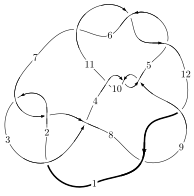
\includegraphics[width=112pt]{../../../GIT/diagram.site/Diagrams/png/1343_12a_0542.png}\\
\ \ \ A knot diagram\footnotemark}&
\allowdisplaybreaks
\textbf{Linearized knot diagam} \\
\cline{2-2}
 &
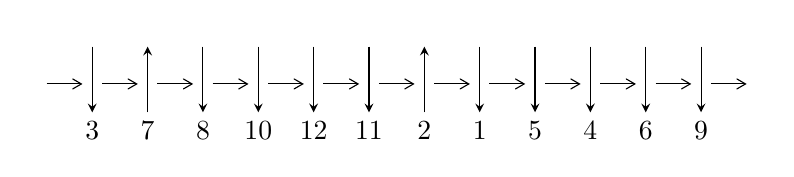
\begin{tikzpicture}[x=20pt, y=17pt]
	% nodes
	\node (C0) at (0, 0) {};
	\node (C1) at (1, 0) {};
	\node (C1U) at (1, +1) {};
	\node (C1D) at (1, -1) {3};

	\node (C2) at (2, 0) {};
	\node (C2U) at (2, +1) {};
	\node (C2D) at (2, -1) {7};

	\node (C3) at (3, 0) {};
	\node (C3U) at (3, +1) {};
	\node (C3D) at (3, -1) {8};

	\node (C4) at (4, 0) {};
	\node (C4U) at (4, +1) {};
	\node (C4D) at (4, -1) {10};

	\node (C5) at (5, 0) {};
	\node (C5U) at (5, +1) {};
	\node (C5D) at (5, -1) {12};

	\node (C6) at (6, 0) {};
	\node (C6U) at (6, +1) {};
	\node (C6D) at (6, -1) {11};

	\node (C7) at (7, 0) {};
	\node (C7U) at (7, +1) {};
	\node (C7D) at (7, -1) {2};

	\node (C8) at (8, 0) {};
	\node (C8U) at (8, +1) {};
	\node (C8D) at (8, -1) {1};

	\node (C9) at (9, 0) {};
	\node (C9U) at (9, +1) {};
	\node (C9D) at (9, -1) {5};

	\node (C10) at (10, 0) {};
	\node (C10U) at (10, +1) {};
	\node (C10D) at (10, -1) {4};

	\node (C11) at (11, 0) {};
	\node (C11U) at (11, +1) {};
	\node (C11D) at (11, -1) {6};

	\node (C12) at (12, 0) {};
	\node (C12U) at (12, +1) {};
	\node (C12D) at (12, -1) {9};
	\node (C13) at (13, 0) {};

	% arrows
	\draw[->,>={angle 60}]
	(C0) edge (C1) (C1) edge (C2) (C2) edge (C3) (C3) edge (C4) (C4) edge (C5) (C5) edge (C6) (C6) edge (C7) (C7) edge (C8) (C8) edge (C9) (C9) edge (C10) (C10) edge (C11) (C11) edge (C12) (C12) edge (C13) ;	\draw[->,>=stealth]
	(C1U) edge (C1D) (C2D) edge (C2U) (C3U) edge (C3D) (C4U) edge (C4D) (C5U) edge (C5D) (C6U) edge (C6D) (C7D) edge (C7U) (C8U) edge (C8D) (C9U) edge (C9D) (C10U) edge (C10D) (C11U) edge (C11D) (C12U) edge (C12D) ;
	\end{tikzpicture} \\
\hhline{~~} \\& 
\textbf{Solving Sequence} \\ \cline{2-2} 
 &
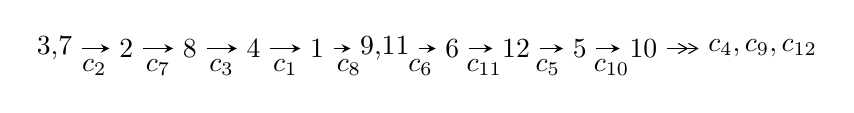
\begin{tikzpicture}[x=23pt, y=7pt]
	% node
	\node (A0) at (-1/8, 0) {3,7};
	\node (A1) at (1, 0) {2};
	\node (A2) at (2, 0) {8};
	\node (A3) at (3, 0) {4};
	\node (A4) at (4, 0) {1};
	\node (A5) at (81/16, 0) {9,11};
	\node (A6) at (49/8, 0) {6};
	\node (A7) at (57/8, 0) {12};
	\node (A8) at (65/8, 0) {5};
	\node (A9) at (73/8, 0) {10};
	\node (C1) at (1/2, -1) {$c_{2}$};
	\node (C2) at (3/2, -1) {$c_{7}$};
	\node (C3) at (5/2, -1) {$c_{3}$};
	\node (C4) at (7/2, -1) {$c_{1}$};
	\node (C5) at (9/2, -1) {$c_{8}$};
	\node (C6) at (45/8, -1) {$c_{6}$};
	\node (C7) at (53/8, -1) {$c_{11}$};
	\node (C8) at (61/8, -1) {$c_{5}$};
	\node (C9) at (69/8, -1) {$c_{10}$};
	\node (A10) at (11, 0) {$c_{4},c_{9},c_{12}$};

	% edge
	\draw[->,>=stealth]	
	(A0) edge (A1) (A1) edge (A2) (A2) edge (A3) (A3) edge (A4) (A4) edge (A5) (A5) edge (A6) (A6) edge (A7) (A7) edge (A8) (A8) edge (A9) ;
	\draw[->>,>={angle 60}]	
	(A9) edge (A10);
\end{tikzpicture} \\ 

\end{tabular} \\

\footnotetext{
The image of knot diagram is generated by the software ``\textbf{Draw programme}" developed by Andrew Bartholomew(\url{http://www.layer8.co.uk/maths/draw/index.htm\#Running-draw}), where we modified some parts for our purpose(\url{https://github.com/CATsTAILs/LinksPainter}).
}\phantom \\ \newline 
\centering \textbf{Ideals for irreducible components\footnotemark of $X_{\text{par}}$} 
 
\begin{align*}
I^u_{1}&=\langle 
2 u^{32}-7 u^{31}+\cdots+b+5,\;- u^{32}+u^{31}+\cdots+2 a-5,\;u^{33}-3 u^{32}+\cdots+11 u-2\rangle \\
I^u_{2}&=\langle 
- u^{18} a+u^{18}+\cdots+b- a,\;u^{19}- u^{17} a+\cdots+a^2-1,\;u^{20}+u^{19}+\cdots+2 u+1\rangle \\
I^u_{3}&=\langle 
- u^{11}-2 u^9+u^8-3 u^7+2 u^6- u^5+2 u^4+u^2+b,\;- u^{10}-2 u^8-2 u^6+u^2+a,\\
\phantom{I^u_{3}}&\phantom{= \langle  }u^{12}+3 u^{10}+5 u^8+4 u^6+2 u^4+u^2+1\rangle \\
\\
\end{align*}
\raggedright * 3 irreducible components of $\dim_{\mathbb{C}}=0$, with total 85 representations.\\
\footnotetext{All coefficients of polynomials are rational numbers. But the coefficients are sometimes approximated in decimal forms when there is not enough margin.}
\newpage
\renewcommand{\arraystretch}{1}
\centering \section*{I. $I^u_{1}= \langle 2 u^{32}-7 u^{31}+\cdots+b+5,\;- u^{32}+u^{31}+\cdots+2 a-5,\;u^{33}-3 u^{32}+\cdots+11 u-2 \rangle$}
\flushleft \textbf{(i) Arc colorings}\\
\begin{tabular}{m{7pt} m{180pt} m{7pt} m{180pt} }
\flushright $a_{3}=$&$\begin{pmatrix}1\\0\end{pmatrix}$ \\
\flushright $a_{7}=$&$\begin{pmatrix}0\\u\end{pmatrix}$ \\
\flushright $a_{2}=$&$\begin{pmatrix}1\\u^2\end{pmatrix}$ \\
\flushright $a_{8}=$&$\begin{pmatrix}u\\u^3+u\end{pmatrix}$ \\
\flushright $a_{4}=$&$\begin{pmatrix}u^4+u^2+1\\u^6+2 u^4+u^2\end{pmatrix}$ \\
\flushright $a_{1}=$&$\begin{pmatrix}u^2+1\\u^2\end{pmatrix}$ \\
\flushright $a_{9}=$&$\begin{pmatrix}- u^7-2 u^5-2 u^3\\- u^7- u^5+u\end{pmatrix}$ \\
\flushright $a_{11}=$&$\begin{pmatrix}\frac{1}{2} u^{32}-\frac{1}{2} u^{31}+\cdots-5 u+\frac{5}{2}\\-2 u^{32}+7 u^{31}+\cdots+26 u-5\end{pmatrix}$ \\
\flushright $a_{6}=$&$\begin{pmatrix}\frac{1}{2} u^{32}-\frac{3}{2} u^{31}+\cdots-6 u+\frac{3}{2}\\u^{30}- u^{29}+\cdots-3 u+1\end{pmatrix}$ \\
\flushright $a_{12}=$&$\begin{pmatrix}u^{12}+3 u^{10}+5 u^8+4 u^6+2 u^4+u^2+1\\u^{12}+2 u^{10}+2 u^8- u^4\end{pmatrix}$ \\
\flushright $a_{5}=$&$\begin{pmatrix}\frac{3}{2} u^{32}-\frac{9}{2} u^{31}+\cdots-18 u+\frac{9}{2}\\- u^{31}+3 u^{30}+\cdots-12 u+3\end{pmatrix}$ \\
\flushright $a_{10}=$&$\begin{pmatrix}\frac{1}{2} u^{32}-\frac{1}{2} u^{31}+\cdots-4 u+\frac{3}{2}\\- u^{32}+4 u^{31}+\cdots+15 u-3\end{pmatrix}$\\&\end{tabular}
\flushleft \textbf{(ii) Obstruction class $= -1$}\\~\\
\flushleft \textbf{(iii) Cusp Shapes $= 2 u^{32}-6 u^{31}+18 u^{30}-40 u^{29}+72 u^{28}-142 u^{27}+192 u^{26}-340 u^{25}+374 u^{24}-594 u^{23}+574 u^{22}-810 u^{21}+724 u^{20}-894 u^{19}+758 u^{18}-840 u^{17}+664 u^{16}-680 u^{15}+466 u^{14}-448 u^{13}+262 u^{12}-214 u^{11}+100 u^{10}-42 u^9-6 u^8+20 u^7-48 u^6+34 u^5-38 u^4+36 u^3-20 u^2+26 u-22$}\\~\\
\newpage\renewcommand{\arraystretch}{1}
\flushleft \textbf{(iv) u-Polynomials at the component}\newline \\
\begin{tabular}{m{50pt}|m{274pt}}
Crossings & \hspace{64pt}u-Polynomials at each crossing \\
\hline $$\begin{aligned}c_{1}\end{aligned}$$&$\begin{aligned}
&u^{33}+15 u^{32}+\cdots+9 u-4
\end{aligned}$\\
\hline $$\begin{aligned}c_{2},c_{7}\end{aligned}$$&$\begin{aligned}
&u^{33}+3 u^{32}+\cdots+11 u+2
\end{aligned}$\\
\hline $$\begin{aligned}c_{3}\end{aligned}$$&$\begin{aligned}
&u^{33}-3 u^{32}+\cdots-73 u+10
\end{aligned}$\\
\hline $$\begin{aligned}c_{4},c_{5},c_{6}\\c_{9},c_{10},c_{11}\end{aligned}$$&$\begin{aligned}
&u^{33}+22 u^{31}+\cdots+3 u+1
\end{aligned}$\\
\hline $$\begin{aligned}c_{8},c_{12}\end{aligned}$$&$\begin{aligned}
&u^{33}+15 u^{32}+\cdots+2771 u+266
\end{aligned}$\\
\hline
\end{tabular}\\~\\
\newpage\renewcommand{\arraystretch}{1}
\flushleft \textbf{(v) Riley Polynomials at the component}\newline \\
\begin{tabular}{m{50pt}|m{274pt}}
Crossings & \hspace{64pt}Riley Polynomials at each crossing \\
\hline $$\begin{aligned}c_{1}\end{aligned}$$&$\begin{aligned}
&y^{33}+7 y^{32}+\cdots+561 y-16
\end{aligned}$\\
\hline $$\begin{aligned}c_{2},c_{7}\end{aligned}$$&$\begin{aligned}
&y^{33}+15 y^{32}+\cdots+9 y-4
\end{aligned}$\\
\hline $$\begin{aligned}c_{3}\end{aligned}$$&$\begin{aligned}
&y^{33}- y^{32}+\cdots+2089 y-100
\end{aligned}$\\
\hline $$\begin{aligned}c_{4},c_{5},c_{6}\\c_{9},c_{10},c_{11}\end{aligned}$$&$\begin{aligned}
&y^{33}+44 y^{32}+\cdots-9 y-1
\end{aligned}$\\
\hline $$\begin{aligned}c_{8},c_{12}\end{aligned}$$&$\begin{aligned}
&y^{33}+27 y^{32}+\cdots+249593 y-70756
\end{aligned}$\\
\hline
\end{tabular}\\~\\
\newpage\flushleft \textbf{(vi) Complex Volumes and Cusp Shapes}
$$\begin{array}{c|c|c}  
\text{Solutions to }I^u_{1}& \I (\text{vol} + \sqrt{-1}CS) & \text{Cusp shape}\\
 \hline 
\begin{aligned}
u &= \phantom{-}0.152282 + 0.979504 I \\
a &= \phantom{-}0.411441 - 0.397281 I \\
b &= -0.351596 - 0.571101 I\end{aligned}
 & -1.33752 - 1.02267 I & -11.79490 + 5.10112 I \\ \hline\begin{aligned}
u &= \phantom{-}0.152282 - 0.979504 I \\
a &= \phantom{-}0.411441 + 0.397281 I \\
b &= -0.351596 + 0.571101 I\end{aligned}
 & -1.33752 + 1.02267 I & -11.79490 - 5.10112 I \\ \hline\begin{aligned}
u &= -0.792598 + 0.556744 I \\
a &= \phantom{-}0.72926 - 1.56216 I \\
b &= -0.99765 - 2.35854 I\end{aligned}
 & \phantom{-}18.0990 - 6.1471 I & \phantom{-}1.69208 + 3.47910 I \\ \hline\begin{aligned}
u &= -0.792598 - 0.556744 I \\
a &= \phantom{-}0.72926 + 1.56216 I \\
b &= -0.99765 + 2.35854 I\end{aligned}
 & \phantom{-}18.0990 + 6.1471 I & \phantom{-}1.69208 - 3.47910 I \\ \hline\begin{aligned}
u &= -0.650620 + 0.804954 I \\
a &= -1.19586 + 1.00059 I \\
b &= \phantom{-}0.77206 + 2.17268 I\end{aligned}
 & \phantom{-}12.43520 - 2.51799 I & \phantom{-}1.14659 + 3.10078 I \\ \hline\begin{aligned}
u &= -0.650620 - 0.804954 I \\
a &= -1.19586 - 1.00059 I \\
b &= \phantom{-}0.77206 - 2.17268 I\end{aligned}
 & \phantom{-}12.43520 + 2.51799 I & \phantom{-}1.14659 - 3.10078 I \\ \hline\begin{aligned}
u &= -0.312053 + 0.912696 I \\
a &= \phantom{-}0.330741 - 0.254799 I \\
b &= -0.282384 - 0.391510 I\end{aligned}
 & -0.69539 - 1.36266 I & -7.61505 + 4.53766 I \\ \hline\begin{aligned}
u &= -0.312053 - 0.912696 I \\
a &= \phantom{-}0.330741 + 0.254799 I \\
b &= -0.282384 + 0.391510 I\end{aligned}
 & -0.69539 + 1.36266 I & -7.61505 - 4.53766 I \\ \hline\begin{aligned}
u &= \phantom{-}0.824879 + 0.434235 I \\
a &= \phantom{-}1.12098 + 1.36653 I \\
b &= -1.46731 + 1.70693 I\end{aligned}
 & \phantom{-}17.3944 - 9.5155 I & \phantom{-}1.10338 + 3.69852 I \\ \hline\begin{aligned}
u &= \phantom{-}0.824879 - 0.434235 I \\
a &= \phantom{-}1.12098 - 1.36653 I \\
b &= -1.46731 - 1.70693 I\end{aligned}
 & \phantom{-}17.3944 + 9.5155 I & \phantom{-}1.10338 - 3.69852 I\\
 \hline 
 \end{array}$$\newpage$$\begin{array}{c|c|c}  
\text{Solutions to }I^u_{1}& \I (\text{vol} + \sqrt{-1}CS) & \text{Cusp shape}\\
 \hline 
\begin{aligned}
u &= \phantom{-}0.431324 + 1.046010 I \\
a &= -0.122761 + 0.496880 I \\
b &= -0.240841 + 1.306230 I\end{aligned}
 & -3.14332 + 3.33428 I & -15.0959 - 5.5855 I \\ \hline\begin{aligned}
u &= \phantom{-}0.431324 - 1.046010 I \\
a &= -0.122761 - 0.496880 I \\
b &= -0.240841 - 1.306230 I\end{aligned}
 & -3.14332 - 3.33428 I & -15.0959 + 5.5855 I \\ \hline\begin{aligned}
u &= \phantom{-}0.726459 + 0.451334 I \\
a &= -0.749693 - 0.212595 I \\
b &= \phantom{-}0.378857 - 0.838797 I\end{aligned}
 & \phantom{-}3.27296 - 2.61780 I & -4.13522 + 5.27122 I \\ \hline\begin{aligned}
u &= \phantom{-}0.726459 - 0.451334 I \\
a &= -0.749693 + 0.212595 I \\
b &= \phantom{-}0.378857 + 0.838797 I\end{aligned}
 & \phantom{-}3.27296 + 2.61780 I & -4.13522 - 5.27122 I \\ \hline\begin{aligned}
u &= -0.707357 + 0.467844 I \\
a &= -0.002391 + 0.722817 I \\
b &= \phantom{-}0.632335 + 0.653593 I\end{aligned}
 & \phantom{-}3.38103 - 0.22806 I & -3.58439 + 4.33946 I \\ \hline\begin{aligned}
u &= -0.707357 - 0.467844 I \\
a &= -0.002391 - 0.722817 I \\
b &= \phantom{-}0.632335 - 0.653593 I\end{aligned}
 & \phantom{-}3.38103 + 0.22806 I & -3.58439 - 4.33946 I \\ \hline\begin{aligned}
u &= \phantom{-}0.088747 + 1.156850 I \\
a &= -1.388160 + 0.151770 I \\
b &= \phantom{-}0.022859 + 0.945454 I\end{aligned}
 & \phantom{-}11.90350 - 7.25131 I & -4.54406 + 3.22535 I \\ \hline\begin{aligned}
u &= \phantom{-}0.088747 - 1.156850 I \\
a &= -1.388160 - 0.151770 I \\
b &= \phantom{-}0.022859 - 0.945454 I\end{aligned}
 & \phantom{-}11.90350 + 7.25131 I & -4.54406 - 3.22535 I \\ \hline\begin{aligned}
u &= \phantom{-}0.318246 + 1.146590 I \\
a &= \phantom{-}1.217500 + 0.275354 I \\
b &= \phantom{-}1.209060 + 0.038598 I\end{aligned}
 & \phantom{-}5.45646 - 0.34796 I & -5.32880 - 0.36416 I \\ \hline\begin{aligned}
u &= \phantom{-}0.318246 - 1.146590 I \\
a &= \phantom{-}1.217500 - 0.275354 I \\
b &= \phantom{-}1.209060 - 0.038598 I\end{aligned}
 & \phantom{-}5.45646 + 0.34796 I & -5.32880 + 0.36416 I\\
 \hline 
 \end{array}$$\newpage$$\begin{array}{c|c|c}  
\text{Solutions to }I^u_{1}& \I (\text{vol} + \sqrt{-1}CS) & \text{Cusp shape}\\
 \hline 
\begin{aligned}
u &= -0.580137 + 1.064780 I \\
a &= -0.502160 + 0.001706 I \\
b &= -0.032476 + 0.816149 I\end{aligned}
 & \phantom{-}1.61599 - 4.72097 I & -6.74809 + 0.86070 I \\ \hline\begin{aligned}
u &= -0.580137 - 1.064780 I \\
a &= -0.502160 - 0.001706 I \\
b &= -0.032476 - 0.816149 I\end{aligned}
 & \phantom{-}1.61599 + 4.72097 I & -6.74809 - 0.86070 I \\ \hline\begin{aligned}
u &= \phantom{-}0.589459 + 1.075110 I \\
a &= -0.159012 - 0.548760 I \\
b &= \phantom{-}0.88162 - 1.58124 I\end{aligned}
 & \phantom{-}1.43372 + 7.64854 I & -7.35632 - 9.80003 I \\ \hline\begin{aligned}
u &= \phantom{-}0.589459 - 1.075110 I \\
a &= -0.159012 + 0.548760 I \\
b &= \phantom{-}0.88162 + 1.58124 I\end{aligned}
 & \phantom{-}1.43372 - 7.64854 I & -7.35632 + 9.80003 I \\ \hline\begin{aligned}
u &= -0.653412 + 1.040510 I \\
a &= \phantom{-}1.258390 - 0.530338 I \\
b &= -0.66209 - 2.26242 I\end{aligned}
 & \phantom{-}16.6529 + 0.7161 I & -0.27219 + 1.44446 I \\ \hline\begin{aligned}
u &= -0.653412 - 1.040510 I \\
a &= \phantom{-}1.258390 + 0.530338 I \\
b &= -0.66209 + 2.26242 I\end{aligned}
 & \phantom{-}16.6529 - 0.7161 I & -0.27219 - 1.44446 I \\ \hline\begin{aligned}
u &= \phantom{-}0.736931 + 0.188573 I \\
a &= -0.64087 - 1.89931 I \\
b &= \phantom{-}0.664431 - 0.704418 I\end{aligned}
 & \phantom{-}9.45531 - 3.71600 I & -0.33346 + 2.59966 I \\ \hline\begin{aligned}
u &= \phantom{-}0.736931 - 0.188573 I \\
a &= -0.64087 + 1.89931 I \\
b &= \phantom{-}0.664431 + 0.704418 I\end{aligned}
 & \phantom{-}9.45531 + 3.71600 I & -0.33346 - 2.59966 I \\ \hline\begin{aligned}
u &= \phantom{-}0.504676 + 1.139920 I \\
a &= -1.045940 - 0.587726 I \\
b &= -1.15935 - 2.28346 I\end{aligned}
 & \phantom{-}6.69649 + 8.32618 I & -3.83980 - 6.48439 I \\ \hline\begin{aligned}
u &= \phantom{-}0.504676 - 1.139920 I \\
a &= -1.045940 + 0.587726 I \\
b &= -1.15935 + 2.28346 I\end{aligned}
 & \phantom{-}6.69649 - 8.32618 I & -3.83980 + 6.48439 I\\
 \hline 
 \end{array}$$\newpage$$\begin{array}{c|c|c}  
\text{Solutions to }I^u_{1}& \I (\text{vol} + \sqrt{-1}CS) & \text{Cusp shape}\\
 \hline 
\begin{aligned}
u &= \phantom{-}0.623116 + 1.112210 I \\
a &= \phantom{-}0.964833 + 0.850517 I \\
b &= -0.28596 + 3.70200 I\end{aligned}
 & \phantom{-}15.3636 + 14.9191 I & -1.64706 - 7.93751 I \\ \hline\begin{aligned}
u &= \phantom{-}0.623116 - 1.112210 I \\
a &= \phantom{-}0.964833 - 0.850517 I \\
b &= -0.28596 - 3.70200 I\end{aligned}
 & \phantom{-}15.3636 - 14.9191 I & -1.64706 + 7.93751 I \\ \hline\begin{aligned}
u &= \phantom{-}0.400115\phantom{ +0.000000I} \\
a &= \phantom{-}1.04742\phantom{ +0.000000I} \\
b &= -0.163122\phantom{ +0.000000I}\end{aligned}
 & -0.742996\phantom{ +0.000000I} & -13.2940\phantom{ +0.000000I}\\
 \hline 
 \end{array}$$\newpage\newpage\renewcommand{\arraystretch}{1}
\centering \section*{II. $I^u_{2}= \langle - u^{18} a+u^{18}+\cdots+b- a,\;u^{19}- u^{17} a+\cdots+a^2-1,\;u^{20}+u^{19}+\cdots+2 u+1 \rangle$}
\flushleft \textbf{(i) Arc colorings}\\
\begin{tabular}{m{7pt} m{180pt} m{7pt} m{180pt} }
\flushright $a_{3}=$&$\begin{pmatrix}1\\0\end{pmatrix}$ \\
\flushright $a_{7}=$&$\begin{pmatrix}0\\u\end{pmatrix}$ \\
\flushright $a_{2}=$&$\begin{pmatrix}1\\u^2\end{pmatrix}$ \\
\flushright $a_{8}=$&$\begin{pmatrix}u\\u^3+u\end{pmatrix}$ \\
\flushright $a_{4}=$&$\begin{pmatrix}u^4+u^2+1\\u^6+2 u^4+u^2\end{pmatrix}$ \\
\flushright $a_{1}=$&$\begin{pmatrix}u^2+1\\u^2\end{pmatrix}$ \\
\flushright $a_{9}=$&$\begin{pmatrix}- u^7-2 u^5-2 u^3\\- u^7- u^5+u\end{pmatrix}$ \\
\flushright $a_{11}=$&$\begin{pmatrix}a\\u^{18} a- u^{18}+\cdots+2 a u+a\end{pmatrix}$ \\
\flushright $a_{6}=$&$\begin{pmatrix}u^{18} a+u^{19}+\cdots+3 u+1\\- u^{19} a+u^{19}+\cdots+2 u^2+u\end{pmatrix}$ \\
\flushright $a_{12}=$&$\begin{pmatrix}u^{12}+3 u^{10}+5 u^8+4 u^6+2 u^4+u^2+1\\u^{12}+2 u^{10}+2 u^8- u^4\end{pmatrix}$ \\
\flushright $a_{5}=$&$\begin{pmatrix}u^{18} a+u^{19}+\cdots+3 u+1\\- u^{19} a+u^{19}+\cdots+2 u^2+u\end{pmatrix}$ \\
\flushright $a_{10}=$&$\begin{pmatrix}u^{17}+4 u^{15}+\cdots+a+1\\u^{18} a- u^{18}+\cdots+a- u\end{pmatrix}$\\&\end{tabular}
\flushleft \textbf{(ii) Obstruction class $= -1$}\\~\\
\flushleft \textbf{(iii) Cusp Shapes $= -4 u^{18}-4 u^{17}-16 u^{16}-16 u^{15}-36 u^{14}-40 u^{13}-52 u^{12}-60 u^{11}-56 u^{10}-64 u^9-56 u^8-52 u^7-48 u^6-40 u^5-32 u^4-32 u^3-12 u^2-12 u-10$}\\~\\
\newpage\renewcommand{\arraystretch}{1}
\flushleft \textbf{(iv) u-Polynomials at the component}\newline \\
\begin{tabular}{m{50pt}|m{274pt}}
Crossings & \hspace{64pt}u-Polynomials at each crossing \\
\hline $$\begin{aligned}c_{1}\end{aligned}$$&$\begin{aligned}
&(u^{20}+9 u^{19}+\cdots+2 u+1)^{2}
\end{aligned}$\\
\hline $$\begin{aligned}c_{2},c_{7}\end{aligned}$$&$\begin{aligned}
&(u^{20}- u^{19}+\cdots-2 u+1)^{2}
\end{aligned}$\\
\hline $$\begin{aligned}c_{3}\end{aligned}$$&$\begin{aligned}
&(u^{20}+u^{19}+\cdots+4 u+1)^{2}
\end{aligned}$\\
\hline $$\begin{aligned}c_{4},c_{5},c_{6}\\c_{9},c_{10},c_{11}\end{aligned}$$&$\begin{aligned}
&u^{40}- u^{39}+\cdots+66 u+17
\end{aligned}$\\
\hline $$\begin{aligned}c_{8},c_{12}\end{aligned}$$&$\begin{aligned}
&(u^{20}-5 u^{19}+\cdots-2 u+1)^{2}
\end{aligned}$\\
\hline
\end{tabular}\\~\\
\newpage\renewcommand{\arraystretch}{1}
\flushleft \textbf{(v) Riley Polynomials at the component}\newline \\
\begin{tabular}{m{50pt}|m{274pt}}
Crossings & \hspace{64pt}Riley Polynomials at each crossing \\
\hline $$\begin{aligned}c_{1}\end{aligned}$$&$\begin{aligned}
&(y^{20}+5 y^{19}+\cdots+10 y+1)^{2}
\end{aligned}$\\
\hline $$\begin{aligned}c_{2},c_{7}\end{aligned}$$&$\begin{aligned}
&(y^{20}+9 y^{19}+\cdots+2 y+1)^{2}
\end{aligned}$\\
\hline $$\begin{aligned}c_{3}\end{aligned}$$&$\begin{aligned}
&(y^{20}+y^{19}+\cdots+18 y+1)^{2}
\end{aligned}$\\
\hline $$\begin{aligned}c_{4},c_{5},c_{6}\\c_{9},c_{10},c_{11}\end{aligned}$$&$\begin{aligned}
&y^{40}+35 y^{39}+\cdots-140 y+289
\end{aligned}$\\
\hline $$\begin{aligned}c_{8},c_{12}\end{aligned}$$&$\begin{aligned}
&(y^{20}+21 y^{19}+\cdots+10 y+1)^{2}
\end{aligned}$\\
\hline
\end{tabular}\\~\\
\newpage\flushleft \textbf{(vi) Complex Volumes and Cusp Shapes}
$$\begin{array}{c|c|c}  
\text{Solutions to }I^u_{2}& \I (\text{vol} + \sqrt{-1}CS) & \text{Cusp shape}\\
 \hline 
\begin{aligned}
u &= \phantom{-}0.781348 + 0.506112 I \\
a &= \phantom{-}0.441997 - 1.155880 I \\
b &= \phantom{-}0.856427 - 0.565059 I\end{aligned}
 & \phantom{-}10.37890 + 1.55876 I & \phantom{-}0.11661 - 2.37917 I \\ \hline\begin{aligned}
u &= \phantom{-}0.781348 + 0.506112 I \\
a &= \phantom{-}0.83804 + 1.43690 I \\
b &= -1.33192 + 2.45508 I\end{aligned}
 & \phantom{-}10.37890 + 1.55876 I & \phantom{-}0.11661 - 2.37917 I \\ \hline\begin{aligned}
u &= \phantom{-}0.781348 - 0.506112 I \\
a &= \phantom{-}0.441997 + 1.155880 I \\
b &= \phantom{-}0.856427 + 0.565059 I\end{aligned}
 & \phantom{-}10.37890 - 1.55876 I & \phantom{-}0.11661 + 2.37917 I \\ \hline\begin{aligned}
u &= \phantom{-}0.781348 - 0.506112 I \\
a &= \phantom{-}0.83804 - 1.43690 I \\
b &= -1.33192 - 2.45508 I\end{aligned}
 & \phantom{-}10.37890 - 1.55876 I & \phantom{-}0.11661 + 2.37917 I \\ \hline\begin{aligned}
u &= \phantom{-}0.487491 + 0.960535 I \\
a &= \phantom{-}0.982330 + 0.105300 I \\
b &= -0.201846 - 0.351155 I\end{aligned}
 & \phantom{-}3.03554 + 2.59904 I & -2.40613 - 3.16627 I \\ \hline\begin{aligned}
u &= \phantom{-}0.487491 + 0.960535 I \\
a &= -0.922458 - 0.679240 I \\
b &= \phantom{-}0.64390 - 3.08542 I\end{aligned}
 & \phantom{-}3.03554 + 2.59904 I & -2.40613 - 3.16627 I \\ \hline\begin{aligned}
u &= \phantom{-}0.487491 - 0.960535 I \\
a &= \phantom{-}0.982330 - 0.105300 I \\
b &= -0.201846 + 0.351155 I\end{aligned}
 & \phantom{-}3.03554 - 2.59904 I & -2.40613 + 3.16627 I \\ \hline\begin{aligned}
u &= \phantom{-}0.487491 - 0.960535 I \\
a &= -0.922458 + 0.679240 I \\
b &= \phantom{-}0.64390 + 3.08542 I\end{aligned}
 & \phantom{-}3.03554 - 2.59904 I & -2.40613 + 3.16627 I \\ \hline\begin{aligned}
u &= -0.795114 + 0.464423 I \\
a &= -1.229700 + 0.036323 I \\
b &= \phantom{-}0.103460 + 0.921159 I\end{aligned}
 & \phantom{-}10.14230 + 4.70967 I & -0.36261 - 2.80351 I \\ \hline\begin{aligned}
u &= -0.795114 + 0.464423 I \\
a &= \phantom{-}0.96901 - 1.37386 I \\
b &= -1.62344 - 2.10711 I\end{aligned}
 & \phantom{-}10.14230 + 4.70967 I & -0.36261 - 2.80351 I\\
 \hline 
 \end{array}$$\newpage$$\begin{array}{c|c|c}  
\text{Solutions to }I^u_{2}& \I (\text{vol} + \sqrt{-1}CS) & \text{Cusp shape}\\
 \hline 
\begin{aligned}
u &= -0.795114 - 0.464423 I \\
a &= -1.229700 - 0.036323 I \\
b &= \phantom{-}0.103460 - 0.921159 I\end{aligned}
 & \phantom{-}10.14230 - 4.70967 I & -0.36261 + 2.80351 I \\ \hline\begin{aligned}
u &= -0.795114 - 0.464423 I \\
a &= \phantom{-}0.96901 + 1.37386 I \\
b &= -1.62344 + 2.10711 I\end{aligned}
 & \phantom{-}10.14230 - 4.70967 I & -0.36261 + 2.80351 I \\ \hline\begin{aligned}
u &= -0.331938 + 1.037100 I \\
a &= \phantom{-}0.990151 - 0.226215 I \\
b &= \phantom{-}0.628424 + 0.095717 I\end{aligned}
 & -0.345495 - 0.748059 I & -11.88926 + 0.17223 I \\ \hline\begin{aligned}
u &= -0.331938 + 1.037100 I \\
a &= -0.226980 - 0.173559 I \\
b &= -1.18881 - 1.01108 I\end{aligned}
 & -0.345495 - 0.748059 I & -11.88926 + 0.17223 I \\ \hline\begin{aligned}
u &= -0.331938 - 1.037100 I \\
a &= \phantom{-}0.990151 + 0.226215 I \\
b &= \phantom{-}0.628424 - 0.095717 I\end{aligned}
 & -0.345495 + 0.748059 I & -11.88926 - 0.17223 I \\ \hline\begin{aligned}
u &= -0.331938 - 1.037100 I \\
a &= -0.226980 + 0.173559 I \\
b &= -1.18881 + 1.01108 I\end{aligned}
 & -0.345495 + 0.748059 I & -11.88926 - 0.17223 I \\ \hline\begin{aligned}
u &= -0.044359 + 1.100970 I \\
a &= \phantom{-}0.572575 + 0.770686 I \\
b &= \phantom{-}0.055517 + 1.140730 I\end{aligned}
 & \phantom{-}4.71375 + 2.89577 I & -6.31229 - 2.74717 I \\ \hline\begin{aligned}
u &= -0.044359 + 1.100970 I \\
a &= -1.352650 - 0.043914 I \\
b &= \phantom{-}0.686027 - 0.496404 I\end{aligned}
 & \phantom{-}4.71375 + 2.89577 I & -6.31229 - 2.74717 I \\ \hline\begin{aligned}
u &= -0.044359 - 1.100970 I \\
a &= \phantom{-}0.572575 - 0.770686 I \\
b &= \phantom{-}0.055517 - 1.140730 I\end{aligned}
 & \phantom{-}4.71375 - 2.89577 I & -6.31229 + 2.74717 I \\ \hline\begin{aligned}
u &= -0.044359 - 1.100970 I \\
a &= -1.352650 + 0.043914 I \\
b &= \phantom{-}0.686027 + 0.496404 I\end{aligned}
 & \phantom{-}4.71375 - 2.89577 I & -6.31229 + 2.74717 I\\
 \hline 
 \end{array}$$\newpage$$\begin{array}{c|c|c}  
\text{Solutions to }I^u_{2}& \I (\text{vol} + \sqrt{-1}CS) & \text{Cusp shape}\\
 \hline 
\begin{aligned}
u &= -0.502129 + 1.070060 I \\
a &= -0.866977 + 0.566977 I \\
b &= -0.50635 + 2.53990 I\end{aligned}
 & \phantom{-}0.79812 - 6.06247 I & -8.39660 + 7.82928 I \\ \hline\begin{aligned}
u &= -0.502129 + 1.070060 I \\
a &= \phantom{-}0.006209 - 0.502110 I \\
b &= \phantom{-}0.617341 - 1.244530 I\end{aligned}
 & \phantom{-}0.79812 - 6.06247 I & -8.39660 + 7.82928 I \\ \hline\begin{aligned}
u &= -0.502129 - 1.070060 I \\
a &= -0.866977 - 0.566977 I \\
b &= -0.50635 - 2.53990 I\end{aligned}
 & \phantom{-}0.79812 + 6.06247 I & -8.39660 - 7.82928 I \\ \hline\begin{aligned}
u &= -0.502129 - 1.070060 I \\
a &= \phantom{-}0.006209 + 0.502110 I \\
b &= \phantom{-}0.617341 + 1.244530 I\end{aligned}
 & \phantom{-}0.79812 + 6.06247 I & -8.39660 - 7.82928 I \\ \hline\begin{aligned}
u &= \phantom{-}0.455846 + 0.648892 I \\
a &= \phantom{-}0.497045 + 0.987915 I \\
b &= \phantom{-}0.351208 + 1.072320 I\end{aligned}
 & \phantom{-}3.96963 + 1.37271 I & -0.87985 - 4.43993 I \\ \hline\begin{aligned}
u &= \phantom{-}0.455846 + 0.648892 I \\
a &= -1.34650 - 0.83977 I \\
b &= \phantom{-}1.46058 - 1.46134 I\end{aligned}
 & \phantom{-}3.96963 + 1.37271 I & -0.87985 - 4.43993 I \\ \hline\begin{aligned}
u &= \phantom{-}0.455846 - 0.648892 I \\
a &= \phantom{-}0.497045 - 0.987915 I \\
b &= \phantom{-}0.351208 - 1.072320 I\end{aligned}
 & \phantom{-}3.96963 - 1.37271 I & -0.87985 + 4.43993 I \\ \hline\begin{aligned}
u &= \phantom{-}0.455846 - 0.648892 I \\
a &= -1.34650 + 0.83977 I \\
b &= \phantom{-}1.46058 + 1.46134 I\end{aligned}
 & \phantom{-}3.96963 - 1.37271 I & -0.87985 + 4.43993 I \\ \hline\begin{aligned}
u &= \phantom{-}0.628268 + 1.065390 I \\
a &= -0.875257 + 0.344934 I \\
b &= -0.930257 - 0.450510 I\end{aligned}
 & \phantom{-}8.70951 + 3.75485 I & -2.25682 - 2.44199 I \\ \hline\begin{aligned}
u &= \phantom{-}0.628268 + 1.065390 I \\
a &= \phantom{-}1.097080 + 0.604611 I \\
b &= -1.12744 + 2.94413 I\end{aligned}
 & \phantom{-}8.70951 + 3.75485 I & -2.25682 - 2.44199 I\\
 \hline 
 \end{array}$$\newpage$$\begin{array}{c|c|c}  
\text{Solutions to }I^u_{2}& \I (\text{vol} + \sqrt{-1}CS) & \text{Cusp shape}\\
 \hline 
\begin{aligned}
u &= \phantom{-}0.628268 - 1.065390 I \\
a &= -0.875257 - 0.344934 I \\
b &= -0.930257 + 0.450510 I\end{aligned}
 & \phantom{-}8.70951 - 3.75485 I & -2.25682 + 2.44199 I \\ \hline\begin{aligned}
u &= \phantom{-}0.628268 - 1.065390 I \\
a &= \phantom{-}1.097080 - 0.604611 I \\
b &= -1.12744 - 2.94413 I\end{aligned}
 & \phantom{-}8.70951 - 3.75485 I & -2.25682 + 2.44199 I \\ \hline\begin{aligned}
u &= -0.621367 + 1.089770 I \\
a &= -0.010187 + 0.899634 I \\
b &= \phantom{-}1.18418 + 1.91130 I\end{aligned}
 & \phantom{-}8.27570 - 10.03250 I & -3.16919 + 7.28178 I \\ \hline\begin{aligned}
u &= -0.621367 + 1.089770 I \\
a &= \phantom{-}1.005850 - 0.716169 I \\
b &= -0.79344 - 3.61211 I\end{aligned}
 & \phantom{-}8.27570 - 10.03250 I & -3.16919 + 7.28178 I \\ \hline\begin{aligned}
u &= -0.621367 - 1.089770 I \\
a &= -0.010187 - 0.899634 I \\
b &= \phantom{-}1.18418 - 1.91130 I\end{aligned}
 & \phantom{-}8.27570 + 10.03250 I & -3.16919 - 7.28178 I \\ \hline\begin{aligned}
u &= -0.621367 - 1.089770 I \\
a &= \phantom{-}1.005850 + 0.716169 I \\
b &= -0.79344 + 3.61211 I\end{aligned}
 & \phantom{-}8.27570 + 10.03250 I & -3.16919 - 7.28178 I \\ \hline\begin{aligned}
u &= -0.558047 + 0.271580 I \\
a &= \phantom{-}0.923100 - 0.270249 I \\
b &= -0.279531 + 0.414404 I\end{aligned}
 & \phantom{-}2.95992 + 1.83292 I & -4.44386 - 4.26331 I \\ \hline\begin{aligned}
u &= -0.558047 + 0.271580 I \\
a &= -0.99267 + 1.70622 I \\
b &= \phantom{-}0.895968 + 0.669805 I\end{aligned}
 & \phantom{-}2.95992 + 1.83292 I & -4.44386 - 4.26331 I \\ \hline\begin{aligned}
u &= -0.558047 - 0.271580 I \\
a &= \phantom{-}0.923100 + 0.270249 I \\
b &= -0.279531 - 0.414404 I\end{aligned}
 & \phantom{-}2.95992 - 1.83292 I & -4.44386 + 4.26331 I \\ \hline\begin{aligned}
u &= -0.558047 - 0.271580 I \\
a &= -0.99267 - 1.70622 I \\
b &= \phantom{-}0.895968 - 0.669805 I\end{aligned}
 & \phantom{-}2.95992 - 1.83292 I & -4.44386 + 4.26331 I\\
 \hline 
 \end{array}$$\newpage\newpage\renewcommand{\arraystretch}{1}
\centering \section*{III. $I^u_{3}= \langle - u^{11}-2 u^9+\cdots+u^2+b,\;- u^{10}-2 u^8-2 u^6+u^2+a,\;u^{12}+3 u^{10}+5 u^8+4 u^6+2 u^4+u^2+1 \rangle$}
\flushleft \textbf{(i) Arc colorings}\\
\begin{tabular}{m{7pt} m{180pt} m{7pt} m{180pt} }
\flushright $a_{3}=$&$\begin{pmatrix}1\\0\end{pmatrix}$ \\
\flushright $a_{7}=$&$\begin{pmatrix}0\\u\end{pmatrix}$ \\
\flushright $a_{2}=$&$\begin{pmatrix}1\\u^2\end{pmatrix}$ \\
\flushright $a_{8}=$&$\begin{pmatrix}u\\u^3+u\end{pmatrix}$ \\
\flushright $a_{4}=$&$\begin{pmatrix}u^4+u^2+1\\u^6+2 u^4+u^2\end{pmatrix}$ \\
\flushright $a_{1}=$&$\begin{pmatrix}u^2+1\\u^2\end{pmatrix}$ \\
\flushright $a_{9}=$&$\begin{pmatrix}- u^7-2 u^5-2 u^3\\- u^7- u^5+u\end{pmatrix}$ \\
\flushright $a_{11}=$&$\begin{pmatrix}u^{10}+2 u^8+2 u^6- u^2\\u^{11}+2 u^9- u^8+3 u^7-2 u^6+u^5-2 u^4- u^2\end{pmatrix}$ \\
\flushright $a_{6}=$&$\begin{pmatrix}u^{11}+3 u^9+5 u^7+4 u^5+2 u^3+u\\u^{11}- u^{10}+3 u^9-2 u^8+4 u^7-2 u^6+2 u^5+u-1\end{pmatrix}$ \\
\flushright $a_{12}=$&$\begin{pmatrix}0\\- u^{10}-3 u^8-4 u^6-3 u^4- u^2-1\end{pmatrix}$ \\
\flushright $a_{5}=$&$\begin{pmatrix}u^{11}+3 u^9+5 u^7+4 u^5+2 u^3+u\\u^{11}- u^{10}+3 u^9-2 u^8+4 u^7-2 u^6+2 u^5-1\end{pmatrix}$ \\
\flushright $a_{10}=$&$\begin{pmatrix}u^{10}+2 u^8- u^7+2 u^6-2 u^5-2 u^3- u^2\\u^{11}+2 u^9- u^8+2 u^7-2 u^6-2 u^4- u^2+u\end{pmatrix}$\\&\end{tabular}
\flushleft \textbf{(ii) Obstruction class $= 1$}\\~\\
\flushleft \textbf{(iii) Cusp Shapes $= -4 u^{10}-12 u^8-16 u^6-8 u^4-4$}\\~\\
\newpage\renewcommand{\arraystretch}{1}
\flushleft \textbf{(iv) u-Polynomials at the component}\newline \\
\begin{tabular}{m{50pt}|m{274pt}}
Crossings & \hspace{64pt}u-Polynomials at each crossing \\
\hline $$\begin{aligned}c_{1}\end{aligned}$$&$\begin{aligned}
&(u^6-3 u^5+5 u^4-4 u^3+2 u^2- u+1)^2
\end{aligned}$\\
\hline $$\begin{aligned}c_{2},c_{7},c_{8}\\c_{12}\end{aligned}$$&$\begin{aligned}
&u^{12}+3 u^{10}+5 u^8+4 u^6+2 u^4+u^2+1
\end{aligned}$\\
\hline $$\begin{aligned}c_{3}\end{aligned}$$&$\begin{aligned}
&u^{12}- u^{10}+5 u^8+6 u^4-3 u^2+1
\end{aligned}$\\
\hline $$\begin{aligned}c_{4},c_{5},c_{6}\\c_{9},c_{10},c_{11}\end{aligned}$$&$\begin{aligned}
&(u^2+1)^6
\end{aligned}$\\
\hline
\end{tabular}\\~\\
\newpage\renewcommand{\arraystretch}{1}
\flushleft \textbf{(v) Riley Polynomials at the component}\newline \\
\begin{tabular}{m{50pt}|m{274pt}}
Crossings & \hspace{64pt}Riley Polynomials at each crossing \\
\hline $$\begin{aligned}c_{1}\end{aligned}$$&$\begin{aligned}
&(y^6+y^5+5 y^4+6 y^2+3 y+1)^2
\end{aligned}$\\
\hline $$\begin{aligned}c_{2},c_{7},c_{8}\\c_{12}\end{aligned}$$&$\begin{aligned}
&(y^6+3 y^5+5 y^4+4 y^3+2 y^2+y+1)^2
\end{aligned}$\\
\hline $$\begin{aligned}c_{3}\end{aligned}$$&$\begin{aligned}
&(y^6- y^5+5 y^4+6 y^2-3 y+1)^2
\end{aligned}$\\
\hline $$\begin{aligned}c_{4},c_{5},c_{6}\\c_{9},c_{10},c_{11}\end{aligned}$$&$\begin{aligned}
&(y+1)^{12}
\end{aligned}$\\
\hline
\end{tabular}\\~\\
\newpage\flushleft \textbf{(vi) Complex Volumes and Cusp Shapes}
$$\begin{array}{c|c|c}  
\text{Solutions to }I^u_{3}& \I (\text{vol} + \sqrt{-1}CS) & \text{Cusp shape}\\
 \hline 
\begin{aligned}
u &= \phantom{-}0.295542 + 1.002190 I \\
a &= \phantom{-}0.917982 + 0.270708 I \\
b &= -0.374286 + 1.073090 I\end{aligned}
 & \phantom{-}1.39926 + 0.92430 I & -5.71672 - 0.79423 I \\ \hline\begin{aligned}
u &= \phantom{-}0.295542 - 1.002190 I \\
a &= \phantom{-}0.917982 - 0.270708 I \\
b &= -0.374286 - 1.073090 I\end{aligned}
 & \phantom{-}1.39926 - 0.92430 I & -5.71672 + 0.79423 I \\ \hline\begin{aligned}
u &= -0.295542 + 1.002190 I \\
a &= \phantom{-}0.917982 - 0.270708 I \\
b &= \phantom{-}1.35189 + 0.92878 I\end{aligned}
 & \phantom{-}1.39926 - 0.92430 I & -5.71672 + 0.79423 I \\ \hline\begin{aligned}
u &= -0.295542 - 1.002190 I \\
a &= \phantom{-}0.917982 + 0.270708 I \\
b &= \phantom{-}1.35189 - 0.92878 I\end{aligned}
 & \phantom{-}1.39926 + 0.92430 I & -5.71672 - 0.79423 I \\ \hline\begin{aligned}
u &= \phantom{-}0.664531 + 0.428243 I \\
a &= -0.685196 - 1.063260 I \\
b &= \phantom{-}0.24989 - 1.43772 I\end{aligned}
 & \phantom{-}5.18047 - 0.92430 I & \phantom{-}1.71672 + 0.79423 I \\ \hline\begin{aligned}
u &= \phantom{-}0.664531 - 0.428243 I \\
a &= -0.685196 + 1.063260 I \\
b &= \phantom{-}0.24989 + 1.43772 I\end{aligned}
 & \phantom{-}5.18047 + 0.92430 I & \phantom{-}1.71672 - 0.79423 I \\ \hline\begin{aligned}
u &= -0.664531 + 0.428243 I \\
a &= -0.685196 + 1.063260 I \\
b &= \phantom{-}1.238080 + 0.291690 I\end{aligned}
 & \phantom{-}5.18047 + 0.92430 I & \phantom{-}1.71672 - 0.79423 I \\ \hline\begin{aligned}
u &= -0.664531 - 0.428243 I \\
a &= -0.685196 - 1.063260 I \\
b &= \phantom{-}1.238080 - 0.291690 I\end{aligned}
 & \phantom{-}5.18047 - 0.92430 I & \phantom{-}1.71672 + 0.79423 I \\ \hline\begin{aligned}
u &= \phantom{-}0.558752 + 1.073950 I \\
a &= -0.732786 - 0.381252 I \\
b &= \phantom{-}0.586105 - 1.184950 I\end{aligned}
 & \phantom{-}3.28987 + 5.69302 I & -2.00000 - 5.51057 I \\ \hline\begin{aligned}
u &= \phantom{-}0.558752 - 1.073950 I \\
a &= -0.732786 + 0.381252 I \\
b &= \phantom{-}0.586105 + 1.184950 I\end{aligned}
 & \phantom{-}3.28987 - 5.69302 I & -2.00000 + 5.51057 I\\
 \hline 
 \end{array}$$\newpage$$\begin{array}{c|c|c}  
\text{Solutions to }I^u_{3}& \I (\text{vol} + \sqrt{-1}CS) & \text{Cusp shape}\\
 \hline 
\begin{aligned}
u &= -0.558752 + 1.073950 I \\
a &= -0.732786 + 0.381252 I \\
b &= -1.05168 + 2.33284 I\end{aligned}
 & \phantom{-}3.28987 - 5.69302 I & -2.00000 + 5.51057 I \\ \hline\begin{aligned}
u &= -0.558752 - 1.073950 I \\
a &= -0.732786 - 0.381252 I \\
b &= -1.05168 - 2.33284 I\end{aligned}
 & \phantom{-}3.28987 + 5.69302 I & -2.00000 - 5.51057 I\\
 \hline 
 \end{array}$$\newpage
\newpage\renewcommand{\arraystretch}{1}
\centering \section*{ IV. u-Polynomials}
\begin{tabular}{m{50pt}|m{274pt}}
Crossings & \hspace{64pt}u-Polynomials at each crossing \\
\hline $$\begin{aligned}c_{1}\end{aligned}$$&$\begin{aligned}
&((u^6-3 u^5+5 u^4-4 u^3+2 u^2- u+1)^{2})(u^{20}+9 u^{19}+\cdots+2 u+1)^{2}\\
&\cdot(u^{33}+15 u^{32}+\cdots+9 u-4)
\end{aligned}$\\
\hline $$\begin{aligned}c_{2},c_{7}\end{aligned}$$&$\begin{aligned}
&(u^{12}+3 u^{10}+\cdots+u^2+1)(u^{20}- u^{19}+\cdots-2 u+1)^{2}\\
&\cdot(u^{33}+3 u^{32}+\cdots+11 u+2)
\end{aligned}$\\
\hline $$\begin{aligned}c_{3}\end{aligned}$$&$\begin{aligned}
&(u^{12}- u^{10}+5 u^8+6 u^4-3 u^2+1)(u^{20}+u^{19}+\cdots+4 u+1)^{2}\\
&\cdot(u^{33}-3 u^{32}+\cdots-73 u+10)
\end{aligned}$\\
\hline $$\begin{aligned}c_{4},c_{5},c_{6}\\c_{9},c_{10},c_{11}\end{aligned}$$&$\begin{aligned}
&((u^2+1)^6)(u^{33}+22 u^{31}+\cdots+3 u+1)(u^{40}- u^{39}+\cdots+66 u+17)
\end{aligned}$\\
\hline $$\begin{aligned}c_{8},c_{12}\end{aligned}$$&$\begin{aligned}
&(u^{12}+3 u^{10}+\cdots+u^2+1)(u^{20}-5 u^{19}+\cdots-2 u+1)^{2}\\
&\cdot(u^{33}+15 u^{32}+\cdots+2771 u+266)
\end{aligned}$\\
\hline
\end{tabular}\newpage\renewcommand{\arraystretch}{1}
\centering \section*{ V. Riley Polynomials}
\begin{tabular}{m{50pt}|m{274pt}}
Crossings & \hspace{64pt}Riley Polynomials at each crossing \\
\hline $$\begin{aligned}c_{1}\end{aligned}$$&$\begin{aligned}
&((y^6+y^5+5 y^4+6 y^2+3 y+1)^2)(y^{20}+5 y^{19}+\cdots+10 y+1)^{2}\\
&\cdot(y^{33}+7 y^{32}+\cdots+561 y-16)
\end{aligned}$\\
\hline $$\begin{aligned}c_{2},c_{7}\end{aligned}$$&$\begin{aligned}
&((y^6+3 y^5+5 y^4+4 y^3+2 y^2+y+1)^{2})(y^{20}+9 y^{19}+\cdots+2 y+1)^{2}\\
&\cdot(y^{33}+15 y^{32}+\cdots+9 y-4)
\end{aligned}$\\
\hline $$\begin{aligned}c_{3}\end{aligned}$$&$\begin{aligned}
&((y^6- y^5+5 y^4+6 y^2-3 y+1)^2)(y^{20}+y^{19}+\cdots+18 y+1)^{2}\\
&\cdot(y^{33}- y^{32}+\cdots+2089 y-100)
\end{aligned}$\\
\hline $$\begin{aligned}c_{4},c_{5},c_{6}\\c_{9},c_{10},c_{11}\end{aligned}$$&$\begin{aligned}
&((y+1)^{12})(y^{33}+44 y^{32}+\cdots-9 y-1)(y^{40}+35 y^{39}+\cdots-140 y+289)
\end{aligned}$\\
\hline $$\begin{aligned}c_{8},c_{12}\end{aligned}$$&$\begin{aligned}
&((y^6+3 y^5+5 y^4+4 y^3+2 y^2+y+1)^{2})(y^{20}+21 y^{19}+\cdots+10 y+1)^{2}\\
&\cdot(y^{33}+27 y^{32}+\cdots+249593 y-70756)
\end{aligned}$\\
\hline
\end{tabular}
\vskip 2pc
\end{document}